% Intuition Figure: Why O/R Beats Entropy for Coordination
% This figure demonstrates the key insight: two policies with identical entropy
% can have vastly different coordination potential, which O/R Index captures.

\begin{figure*}[t]
\centering
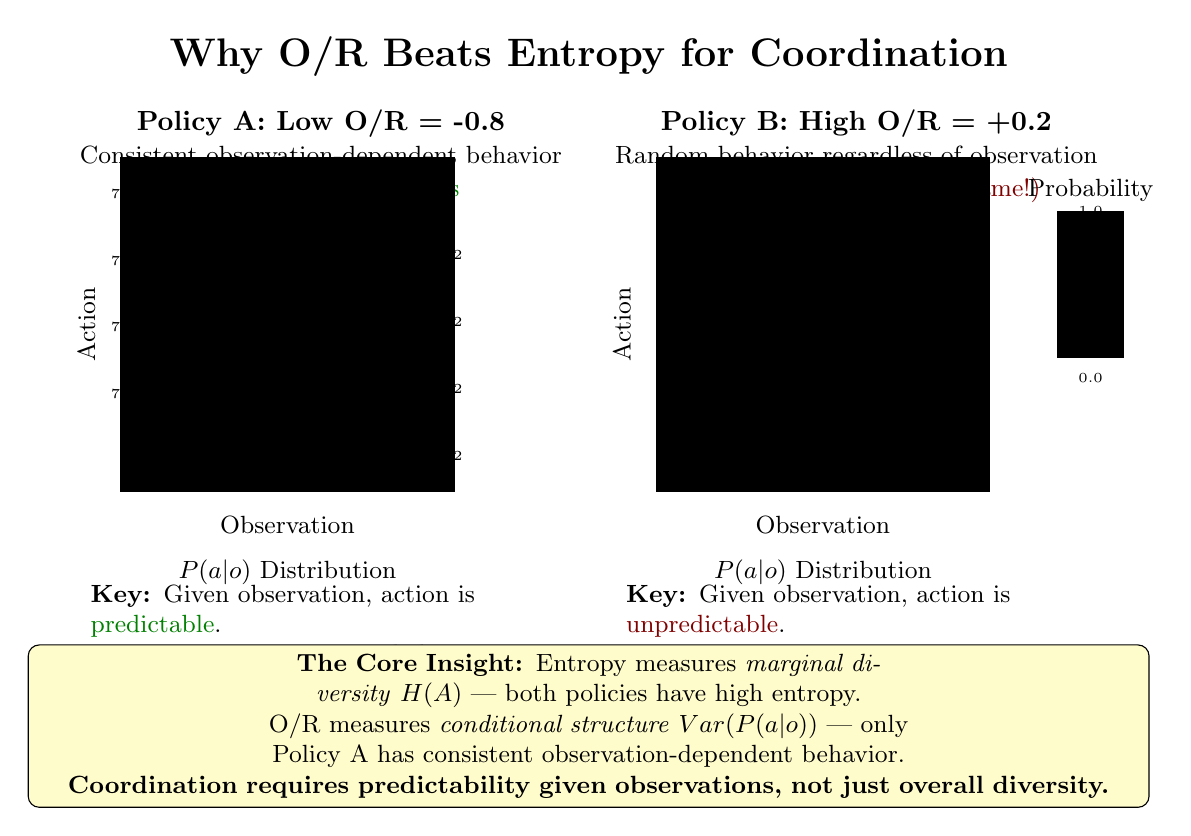
\begin{tikzpicture}[scale=0.85]

% Title for the entire figure
\node[font=\Large\bfseries] at (7, 6.5) {Why O/R Beats Entropy for Coordination};

% LEFT PANEL: Policy A (Good Coordination)
\begin{scope}[shift={(0,0)}]
    % Title
    \node[font=\bfseries, align=center] at (3, 5.5) {Policy A: Low O/R = -0.8};
    \node[font=\small, align=center] at (3, 5.0) {Consistent observation-dependent behavior};
    \node[font=\small, align=center, text=green!50!black] at (3, 4.5) {Entropy H(A) = 1.5 bits};

    % Heatmap grid (5x5 for observations x actions)
    \foreach \i in {0,1,2,3,4} {
        \foreach \j in {0,1,2,3,4} {
            % Create diagonal pattern (strong obs-action dependency)
            \pgfmathsetmacro{\val}{ifthenelse(\i==\j, 0.7, 0.075)}
            \pgfmathsetmacro{\color}{100*\val}
            \fill[blue!\color!white] (\i, \j) rectangle ++(1,1);
            \node[font=\tiny] at (\i+0.5, \j+0.5) {\pgfmathprintnumber[precision=2]{\val}};
        }
    }

    % Axes labels
    \node[font=\small, rotate=90] at (-0.5, 2.5) {Action};
    \node[font=\small] at (2.5, -0.5) {Observation};

    % P(a|o) annotation
    \node[font=\small] at (2.5, -1.2) {$P(a|o)$ Distribution};

    % Key insight annotation
    \node[font=\small, align=left, text width=5cm] at (2.5, -2.2) {
        \textbf{Key:} Given observation, action is \textcolor{green!50!black}{predictable}.\\
        Teammates can anticipate behavior → \textbf{Coordination}
    };
\end{scope}

% RIGHT PANEL: Policy B (Poor Coordination)
\begin{scope}[shift={(8,0)}]
    % Title
    \node[font=\bfseries, align=center] at (3, 5.5) {Policy B: High O/R = +0.2};
    \node[font=\small, align=center] at (3, 5.0) {Random behavior regardless of observation};
    \node[font=\small, align=center, text=red!50!black] at (3, 4.5) {Entropy H(A) = 1.5 bits (same!)};

    % Heatmap grid (5x5 for observations x actions)
    \foreach \i in {0,1,2,3,4} {
        \foreach \j in {0,1,2,3,4} {
            % Create uniform pattern (no obs-action dependency)
            \pgfmathsetmacro{\val}{0.2}
            \pgfmathsetmacro{\color}{100*\val}
            \fill[blue!\color!white] (\i, \j) rectangle ++(1,1);
            \node[font=\tiny] at (\i+0.5, \j+0.5) {0.20};
        }
    }

    % Axes labels
    \node[font=\small, rotate=90] at (-0.5, 2.5) {Action};
    \node[font=\small] at (2.5, -0.5) {Observation};

    % P(a|o) annotation
    \node[font=\small] at (2.5, -1.2) {$P(a|o)$ Distribution};

    % Key insight annotation
    \node[font=\small, align=left, text width=5cm] at (2.5, -2.2) {
        \textbf{Key:} Given observation, action is \textcolor{red!50!black}{unpredictable}.\\
        Teammates cannot anticipate → \textbf{No Coordination}
    };
\end{scope}

% BOTTOM: Key insight box
\node[font=\small, align=center, text width=14cm, draw, fill=yellow!20, rounded corners] at (7, -3.5) {
    \textbf{The Core Insight:} Entropy measures \emph{marginal diversity} $H(A)$ — both policies have high entropy.\\
    O/R measures \emph{conditional structure} $\text{Var}(P(a|o))$ — only Policy A has consistent observation-dependent behavior.\\
    \textbf{Coordination requires predictability given observations, not just overall diversity.}
};

% Color bar legend
\begin{scope}[shift={(14, 2)}]
    \node[font=\small] at (0.5, 2.5) {Probability};
    \foreach \i in {0,...,10} {
        \pgfmathsetmacro{\val}{\i/10}
        \pgfmathsetmacro{\color}{100*\val}
        \fill[blue!\color!white] (0, \i*0.2) rectangle ++(1, 0.2);
    }
    \node[font=\tiny] at (0.5, -0.3) {0.0};
    \node[font=\tiny] at (0.5, 2.2) {1.0};
\end{scope}

\end{tikzpicture}

\caption{\textbf{Why O/R Beats Entropy for Coordination Measurement.}
Two policies with identical action entropy ($H(A) = 1.5$ bits) but vastly different coordination potential.
\textbf{Left (Policy A):} Low O/R Index ($-0.8$) indicates strong conditional structure — actions are predictable given observations (diagonal pattern in $P(a|o)$ heatmap). Teammates can learn to anticipate this agent's behavior, enabling coordination.
\textbf{Right (Policy B):} High O/R Index ($+0.2$) indicates no conditional structure — actions are uniformly random regardless of observations (flat $P(a|o)$ heatmap). Teammates cannot predict behavior, preventing coordination.
Entropy measures marginal diversity; O/R measures conditional consistency — the key to multi-agent coordination.}
\label{fig:or_intuition}
\end{figure*}
